  
\section{Crise de Software}
\begin{frame}
 \frametitle{Crise de Software}
 \begin{itemize}
  \item Termo utilizado nos anos 1970
  %\pause
  \item Expressava as dificuldades do desenvolvimento de software frente ao
  \begin{itemize}
   \item rápido crescimento da demanda por software
   %\pause
   \item   complexidade dos problemas a serem resolvidos
   %\pause
   \item  inexistência de técnicas estabelecidas para o desenvolvimento de sistemas que funcionassem adequadamente
  \end{itemize}
 \end{itemize}
\end{frame}


\begin{frame}[fragile]
 \frametitle{Crise de Software \\ Exemplo - Código Quake III Arena}
 \begin{itemize}
  \item Implementação da raiz quadrada inversa
 \end{itemize}
 \begin{lstlisting}
float Q_rsqrt( float number)
{
  int i;
  float x2, y;
  const float threehalfs = 1.5F;
  x2 = number * 0.5F;
  y = number;
  i = * ( int * ) &y; // evil floating point bit level hacking
  i = 0x5f3759df - ( i >> 1 ); // what the f***?
  y = * ( float * ) &i;
  y = y * ( threehalfs - ( x2 * y * y ) ); // 1st iteration
  return y;
}  
 \end{lstlisting}
\end{frame}

\begin{frame}
\frametitle{Resposta à Crise de Software}
\begin{block}{Processo de Software}
 Abordagem sistemática, disciplinada e possível de
ser medida para o desenvolvimento, operação e manutenção do software
\end{block}
\end{frame}



\begin{frame}
 \frametitle{Processo de Software}
 \begin{block}{}
  Consiste em uma série de atividades, práticas, eventos, ferramentas e
métodos que garantem, técnica e administrativamente que o software
pode ser desenvolvido com qualidade e de maneira \textbf{organizada, disciplinada
e previsível}
 \end{block}
\end{frame}


\begin{frame}
 \frametitle{Processo de Software}
\frametitle{Fases do Processo de Software}
\begin{figure}
 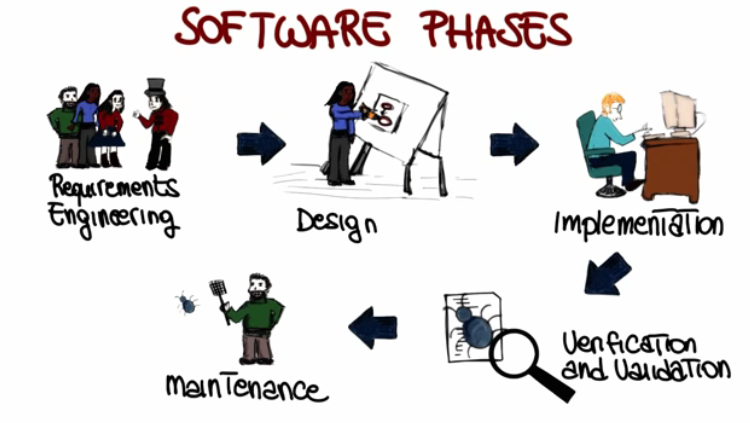
\includegraphics[width = \textwidth]{figs/fig20.png}
\end{figure}
\end{frame}

\begin{frame}
 \frametitle{Requisitos}
 \begin{block}{}
   É o processo para estabelecer quais são as necessidades dos \textit{stakeholders} que devem ser solucionados pelo software
 \end{block}
 \begin{figure}
 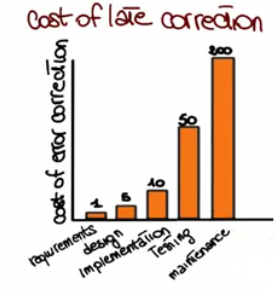
\includegraphics[width = 0.5\textwidth]{figs/fig22.png}
\end{figure}
\end{frame}

\begin{frame}
 \frametitle{Projeto (Design)}
\begin{itemize}
 \item Atividades de projeto:
 \begin{itemize}
  \item Projeto da Arquitetura
  \item Especificação abstrata
  \item Projeto de Interface
  \item Projeto do Componente
  \item Estrutura de dados
  \item Projeto de Arquitetura
 \end{itemize}
\end{itemize}

\end{frame}


\begin{frame}
 \frametitle{Projeto (Design)}
\begin{itemize}
 \item Produtos do Projeto:
 \begin{itemize}
  \item Estrutura do Sistema
  \item Especificação de software
  \item Especificação de Interface
  \item Especificação do Componente
  \item Especificação da Estrutura de dados
  \item Especificação do Algoritmo
 \end{itemize}
\end{itemize}
\end{frame}

\begin{frame}
 \frametitle{Implementação}
\begin{itemize}
 \item Quatro pilares:
 \begin{itemize}
  \item Redução da Complexidade
  \item Antecipar diversidade
  \item Estruturar para validação
  \item Uso de  padrões (interno/externo)
 \end{itemize}
\end{itemize} 
\end{frame}

\begin{frame}
 \frametitle{Verificação e Validação}
\begin{itemize}
 \item \textbf{Validação}:  construimos o sistema correto?
 \item \textbf{Verificação}: construimos o sistema corretamente?
\end{itemize} 
 \begin{figure}
 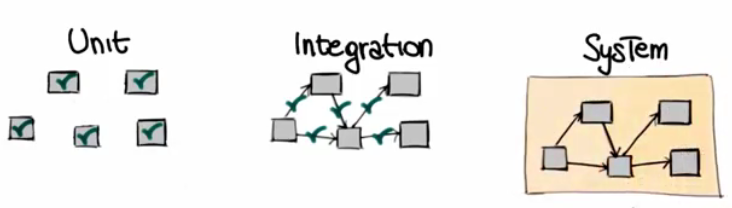
\includegraphics[width = 0.9\textwidth]{figs/fig23.png}
\end{figure}
\end{frame}

\begin{frame}
 \frametitle{Manutenção}

 \begin{figure}
 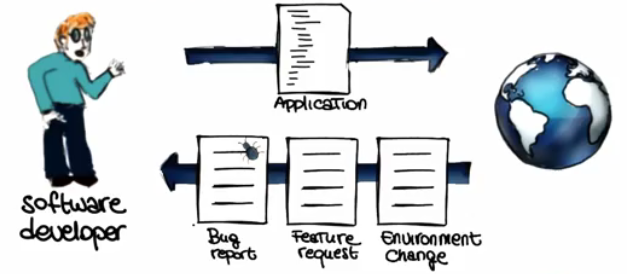
\includegraphics[width =\textwidth]{figs/fig24.png}
\end{figure}
\end{frame}

\begin{frame}
 \frametitle{Processo de Software}
 \begin{block}{Problema}
 Uma das \textbf{maiores dificuldades} encontradas pelas empresas
de software é o \textbf{gerenciamento} de seus \textbf{processos de software}
 \end{block}

 \begin{block}{Solução}
  \textbf{Modelos de Processo de Software}
 \end{block}
\end{frame}

\section{Modelo de Processo}
\begin{frame}
 \frametitle{Modelo de Processo}
 \begin{itemize}
  \item Escolhido de acordo com a natureza da aplicação e as características do projeto
  %\pause
\item Corresponde ao que usualmente se chama de Ciclo de Vida (ISO 9000/3)
%\pause
\item Há vários de modelos de processo de software propostos
 \end{itemize}
\end{frame}

\begin{frame}
 \frametitle{Modelo de Processo}
\begin{figure}
 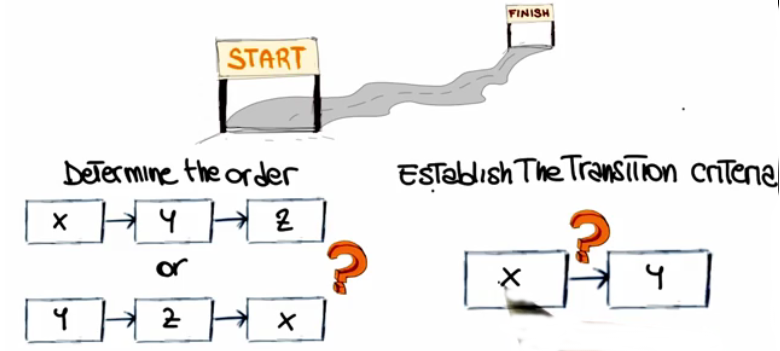
\includegraphics[width = \textwidth]{figs/fig21.png}
\end{figure}
\end{frame}


\begin{frame}
 \frametitle{Modelos de Processo de Software}
 \begin{itemize}
  \item  O Modelo Sequencial Linear
  \begin{itemize}
   \item também chamado Modelo Cascata ou Ciclo de Vida Classico
  \end{itemize}
  %\pause
  \item O Paradigma de Prototipação
  %\pause
  \item O Modelo RAD (Rapid Application Development)
  %\pause
  \item Modelos Evolutivos de Processo de Software
  \begin{itemize}
   \item O Modelo Incremental
   \item O Modelo Espiral
   \item O Modelo de Montagem de Componentes
  \end{itemize}
 \end{itemize}
\end{frame}


\begin{frame}
\frametitle{Modelos de Processo de Software}
 \begin{figure}
  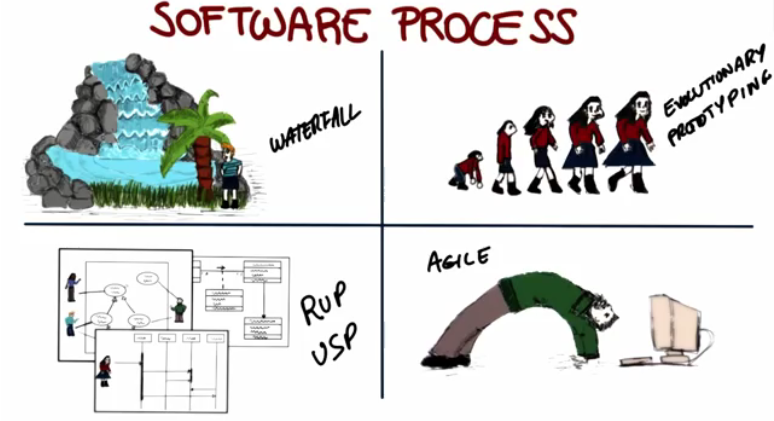
\includegraphics[width = \textwidth]{figs/fig19.png}
 \end{figure}
\end{frame}

\section{Bibliografia}

\begin{frame}
 \frametitle{Bibliografia Sugerida}
 \begin{itemize}
  \item "Construindo Software como Serviço (SaaS): Uma Abordagem Ágil Usando Computação em Nuvem" - Introdução

 \end{itemize}

\end{frame}
% 
